% V3 reusable chapter. Load graphicx and figures/figure_style.tex in the host preamble.
\section{相关工作}
\label{sec:related-work}

食物图像理解包含两个相互关联的目标：将可见内容转化为自然语言，以及将食材组成、份量与营养信息组织为膳食记录。围绕这两个目标，相关研究逐步形成了从视觉表示、序列生成到领域适配和质量评价的方法体系。本节沿四条研究主线梳理代表性进展，为 FoodLens 的自主模型实现与预训练模型适配提供依据。

\subsection{食物图像描述生成研究}
\label{subsec:captioning}
\flfocus{视觉表示由全局向量走向空间 Token，信息交互由循环状态走向注意力与跨层融合。}

\subsubsection{从全局视觉表示到空间注意力}
\textbf{Show and Tell}\cite{vinyals2015show} 将视觉识别与语言生成统一为条件序列建模：预训练 CNN 提取全局图像向量，LSTM 根据图像条件与历史词语逐词生成描述，通过最大化参考句子的条件似然训练。图像在初始时间步输入，后续信息由循环状态传递。该工作在多个数据集上验证了 \textbf{CNN--RNN 编解码范式}，在其 MS COCO 开发集设置下取得 27.7 的 BLEU-4，为从图像到语言的端到端建模建立了清晰起点。

全局向量适合概括场景，食物描述则经常依赖分散的配料、颜色和形态。将整张图像压缩为单一表示，容易弱化多个局部对象及其细微属性。FoodLens 的 \textbf{ResNet-18 + GRU} 延续这一视觉编码与循环解码思路，以轻量骨干和门控循环单元构建自主基线；其设计重点是建立可解释的编码、条件注入和自回归生成流程。原始 Show and Tell 采用 LSTM，GRU 是课程项目对循环解码器的具体选择。

\textbf{Show, Attend and Tell}\cite{xu2015attend} 通过空间注意力将局部视觉信息引入逐词生成。模型保留 VGG-19 的 $14\times14\times512$ 特征网格，根据前一时刻的解码状态计算区域权重，形成动态视觉上下文。软注意力采用可微的区域加权和，硬注意力通过位置采样与随机梯度估计训练。二者都围绕“生成当前词语时关注哪些区域”建立视觉与语言的联系，注意力热图直观呈现这种对应关系。

该论文在 Flickr8k、Flickr30k 和 MS COCO 上验证了注意力机制，软、硬注意力在不同指标上各有优势。\textbf{双随机注意力正则项}鼓励句子生成过程覆盖不同区域，门控系数则调节视觉上下文的使用程度。空间选择缓解了全局压缩的信息瓶颈，也促使后续方法进一步研究区域之间的关系和不同层次视觉信息的组织方式。

\subsubsection{Transformer 与网格特征建模}
Transformer 图像描述模型通过\textbf{自注意力与交叉注意力}连接视觉表示和文本生成：视觉自注意力组织位置之间的关系，文本掩码自注意力建模历史词语，交叉注意力读取视觉上下文。网格特征将卷积特征图组织为视觉 Token，保留局部区域信息，再结合位置表示建模空间关联。训练时各词位置可在给定真实前缀的条件下并行计算，推理时采用自回归生成。

\textbf{Meshed-Memory Transformer}\cite{cornia2020meshed} 同时改进视觉编码和跨层解码。编码器引入可学习的持久记忆向量，解码器通过带门控的网状连接读取多个编码层，从而综合不同层次的区域关系。论文在 COCO Karpathy 划分及在线评测中报告了性能改进。该方法主要采用检测区域特征，其“网状”结构指编码层与解码层之间的连接，为利用多层视觉信息提供了代表性思路。

\textbf{S$^2$ Transformer}\cite{zeng2022s2} 将这一问题推进到网格特征的空间与层次建模。其空间感知伪监督模块（Spatial-aware Pseudo-supervised，\textbf{SP}）学习聚类中心，对网格进行软分配，并聚合相对于中心的残差，形成伪区域特征。原始网格与伪区域由共享参数的编码器处理，在局部覆盖和聚合语义之间形成互补，整个过程使用可学习聚类而无需额外区域标注。

其尺度增强模块（Scale-wise/Scale-aware Reinforcement，\textbf{SR}）拼接不同编码层的输出，经映射与加权残差补充最高层表示，再融合两个分支供解码器使用。SR 的作用是跨层特征融合，序列级奖励训练由独立的训练阶段完成。论文采用来自预训练检测器的 $7\times7\times2048$ 网格输入。在相同 ResNeXt-101 特征、MS COCO Karpathy 测试划分及论文两阶段训练协议下，加入 SP 和 SR 后，CIDEr 由 131.2 提升至 133.5，表列参数量由 33.57M 增至 34.64M，展示了空间聚合与层次融合的收益。

图\ref{fig:s2-architecture}展示 S$^2$ 的实际网络：左侧网格与右侧伪区域经过共享编码，底部 SP 完成空间聚合，两侧 SR 将多层信息补充到解码表示。表\ref{tab:captioning}进一步比较各方法的技术重点。FoodLens 据此设置\textbf{全局特征 + GRU}与\textbf{空间网格 + Transformer}两种自主模型，考察局部信息与注意力建模对食物描述的影响。S$^2$ 为网格模型提供设计依据，M$^2$ 提供多层信息利用的参照；项目比较时结合视觉表示和解码结构两个变化解释结果。

\begin{figure}[!htbp]
 \centering
 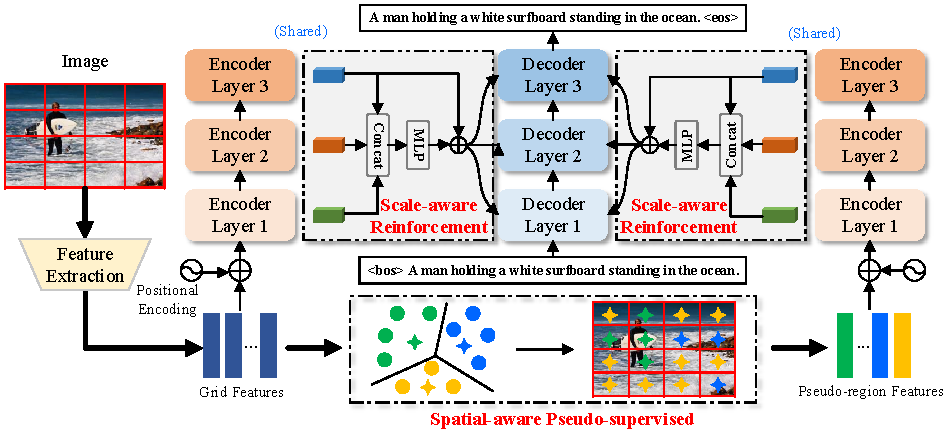
\includegraphics[width=\linewidth]{figures/literature/s2-fig2.pdf}
 \caption{S$^2$ Transformer 的网格与伪区域双分支架构。引自 Zeng 等\cite{zeng2022s2}\href{https://www.ijcai.org/proceedings/2022/0224.pdf}{原图 2（IJCAI）}，裁去页面正文，保留原图连接。SP 聚合网格，SR 融合编码层。}
 \label{fig:s2-architecture}
\end{figure}

\begin{table}[!htbp]
 \caption{图像描述模型的表示与生成方式比较}
 \label{tab:captioning}
 \centering\small
 \setlength{\tabcolsep}{5pt}\renewcommand{\arraystretch}{1.16}
 \begin{tabularx}{\linewidth}{@{}P{3.0cm}P{3.1cm}P{3.15cm}Y@{}}
 \toprule
 \textbf{方法} & \textbf{视觉表示} & \textbf{解码与交互} & \textbf{技术特点}\\
 \midrule
 Show and Tell & CNN 全局向量 & LSTM 循环生成 & 简洁的条件序列基线\\
 Show, Attend and Tell & CNN 空间网格 & 注意力 + LSTM & 逐词选择视觉区域\\
 M$^2$ Transformer & 检测区域、多层编码 & 记忆增强、网状跨层解码 & 综合多层区域关系\\
 S$^2$ Transformer & 原始网格、SP 伪区域 & 共享编码、SR 融合 & 空间聚合与层次互补\\
 \bottomrule
 \end{tabularx}
\end{table}

\subsubsection{细粒度食物描述与领域适配}
\textbf{Food-500 Cap}\cite{ma2023food} 将图像描述评价推进到细粒度食物领域。研究从 ISIA Food-500 的 494 个类别中各选择 50 张图像，共构建 24,700 个图文样本。每张图像对应一条人工描述，覆盖菜品名称、可见食材、颜色、形状和容器，并为类别补充饮食文化来源标签。这类标注将“识别菜品”扩展为“描述区分菜品的可见细节”，与 FoodLens 的任务一直接对应。

该研究以分类、检索、描述和图像合成四种零样本任务探测九种视觉语言模型。描述评价使用 BLEU、METEOR、ROUGE、CIDEr、CLIPScore，以及检查类别名称的\textbf{语义标签准确率}。实验揭示了食物属性遗漏、误识别和不同饮食文化类别的表现差异，说明领域适配与细粒度分析具有实际价值。每图单参考对合理改写的覆盖有限，类别名称匹配侧重菜品识别；FoodLens 因而结合自动指标与食材、属性错误分析评价描述质量，重量和营养标签则由结构化膳食任务提供。

\FloatBarrier
\subsection{食物理解与结构化营养估计研究}
\label{subsec:nutrition}
\flfocus{食材集合回答“有什么”，重量与营养估计回答“有多少”；定量预测依赖可靠的份量监督。}

\subsubsection{食材集合识别与依赖关系}
\textbf{Inverse Cooking}\cite{salvador2019inverse} 以“图像理解—食材预测—食谱生成”组织食物语义推断。模型先从图像预测食材集合，再让步骤解码器同时关注图像特征和食材嵌入。食材预测器利用 Transformer 的自回归过程学习共现关系，以跨时间最大池化后的集合损失减少输出排列的影响，并处理结束标记与集合基数。这种\textbf{依赖建模与集合监督}兼顾了食材间联系和标签的无序性。

在筛选后的 Recipe1M 数据上，论文使用 1,488 项食材词表，测试集全局食材 IoU 和 F1 分别达到 32.11 和 48.61。图像与食材共同生成步骤时，测试困惑度为 8.51，优于仅图像条件的 9.66 和仅食材条件的 8.67，验证了\textbf{视觉信息与显式食材语义的互补性}。该研究的输出是食材集合与食谱，隐藏配料和中间识别错误构成主要困难；将其思想用于膳食记录时，逐食材重量及营养值需要相应的定量标签。

图\ref{fig:inverse-architecture}给出了这一路线的网络结构。食材预测器位于图像编码器与食材编码器之间，步骤解码器接收图像和食材两路表示，将食材识别与语言生成连接起来。

\begin{figure}[!htbp]
 \centering
 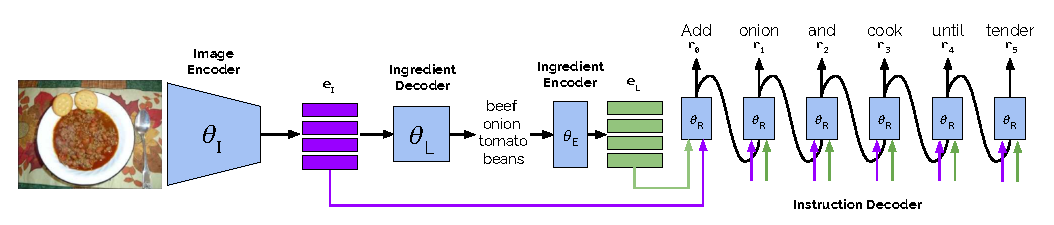
\includegraphics[width=\linewidth]{figures/literature/inverse-cooking-fig2.pdf}
 \caption{Inverse Cooking 的图像、食材与步骤生成网络。引自 Salvador 等\cite{salvador2019inverse}\href{https://openaccess.thecvf.com/content_CVPR_2019/papers/Salvador_Inverse_Cooking_Recipe_Generation_From_Food_Images_CVPR_2019_paper.pdf}{原图 2（CVF）}，仅裁去页面正文；紫色与绿色连接分别传递图像和食材信息。}
 \label{fig:inverse-architecture}
\end{figure}

\subsubsection{份量监督与重量、营养估计}
\textbf{Nutrition5k}\cite{thames2021nutrition} 通过物理测量建立了视觉营养理解的数据基础。论文表 1 列出 5,066 份餐食，涉及超过 250 种食材，约有 20,000 段侧视视频，其中约 3,500 份具有俯视 RGB-D 数据。采集时逐项添加食材或已知配方的成品食物，记录重量增量并扫描；四台侧面摄像机各扫过约 $90^\circ$，共同覆盖餐盘周围视角，俯视 RealSense 提供颜色与深度。

\textbf{增量秤量、配方分解与营养数据库}共同构成标签依据：成品项的食材比例由配方分解，营养值结合食材重量和 USDA 数据库计算。同一餐盘的增量扫描被放入同一数据子集，保持训练与测试之间的餐盘独立性。

Nutrition5k 的主要基线采用 \textbf{InceptionV2 多任务回归}，通过共享视觉特征和任务分支预测热量、宏量营养素以及需要时的总重量，训练与评价主要使用 MAE。论文区分了\textbf{每克营养密度}与\textbf{整餐绝对值}：前者按真实重量归一化标签，并在表中借助真实重量换算为整餐数值；后者直接从 RGB 预测总量，同时承担组成识别与份量估计。数据提供食材级重量，主要回归基线关注整餐级输出。

图\ref{fig:nutrition-architecture}展示共享骨干与多个回归头的连接方式。与图\ref{fig:inverse-architecture}的食材条件生成相比，这一架构将视觉表示直接映射为重量及营养数值，训练监督也相应转向物理测量和数据库标签。

\begin{figure}[!htbp]
 \centering
 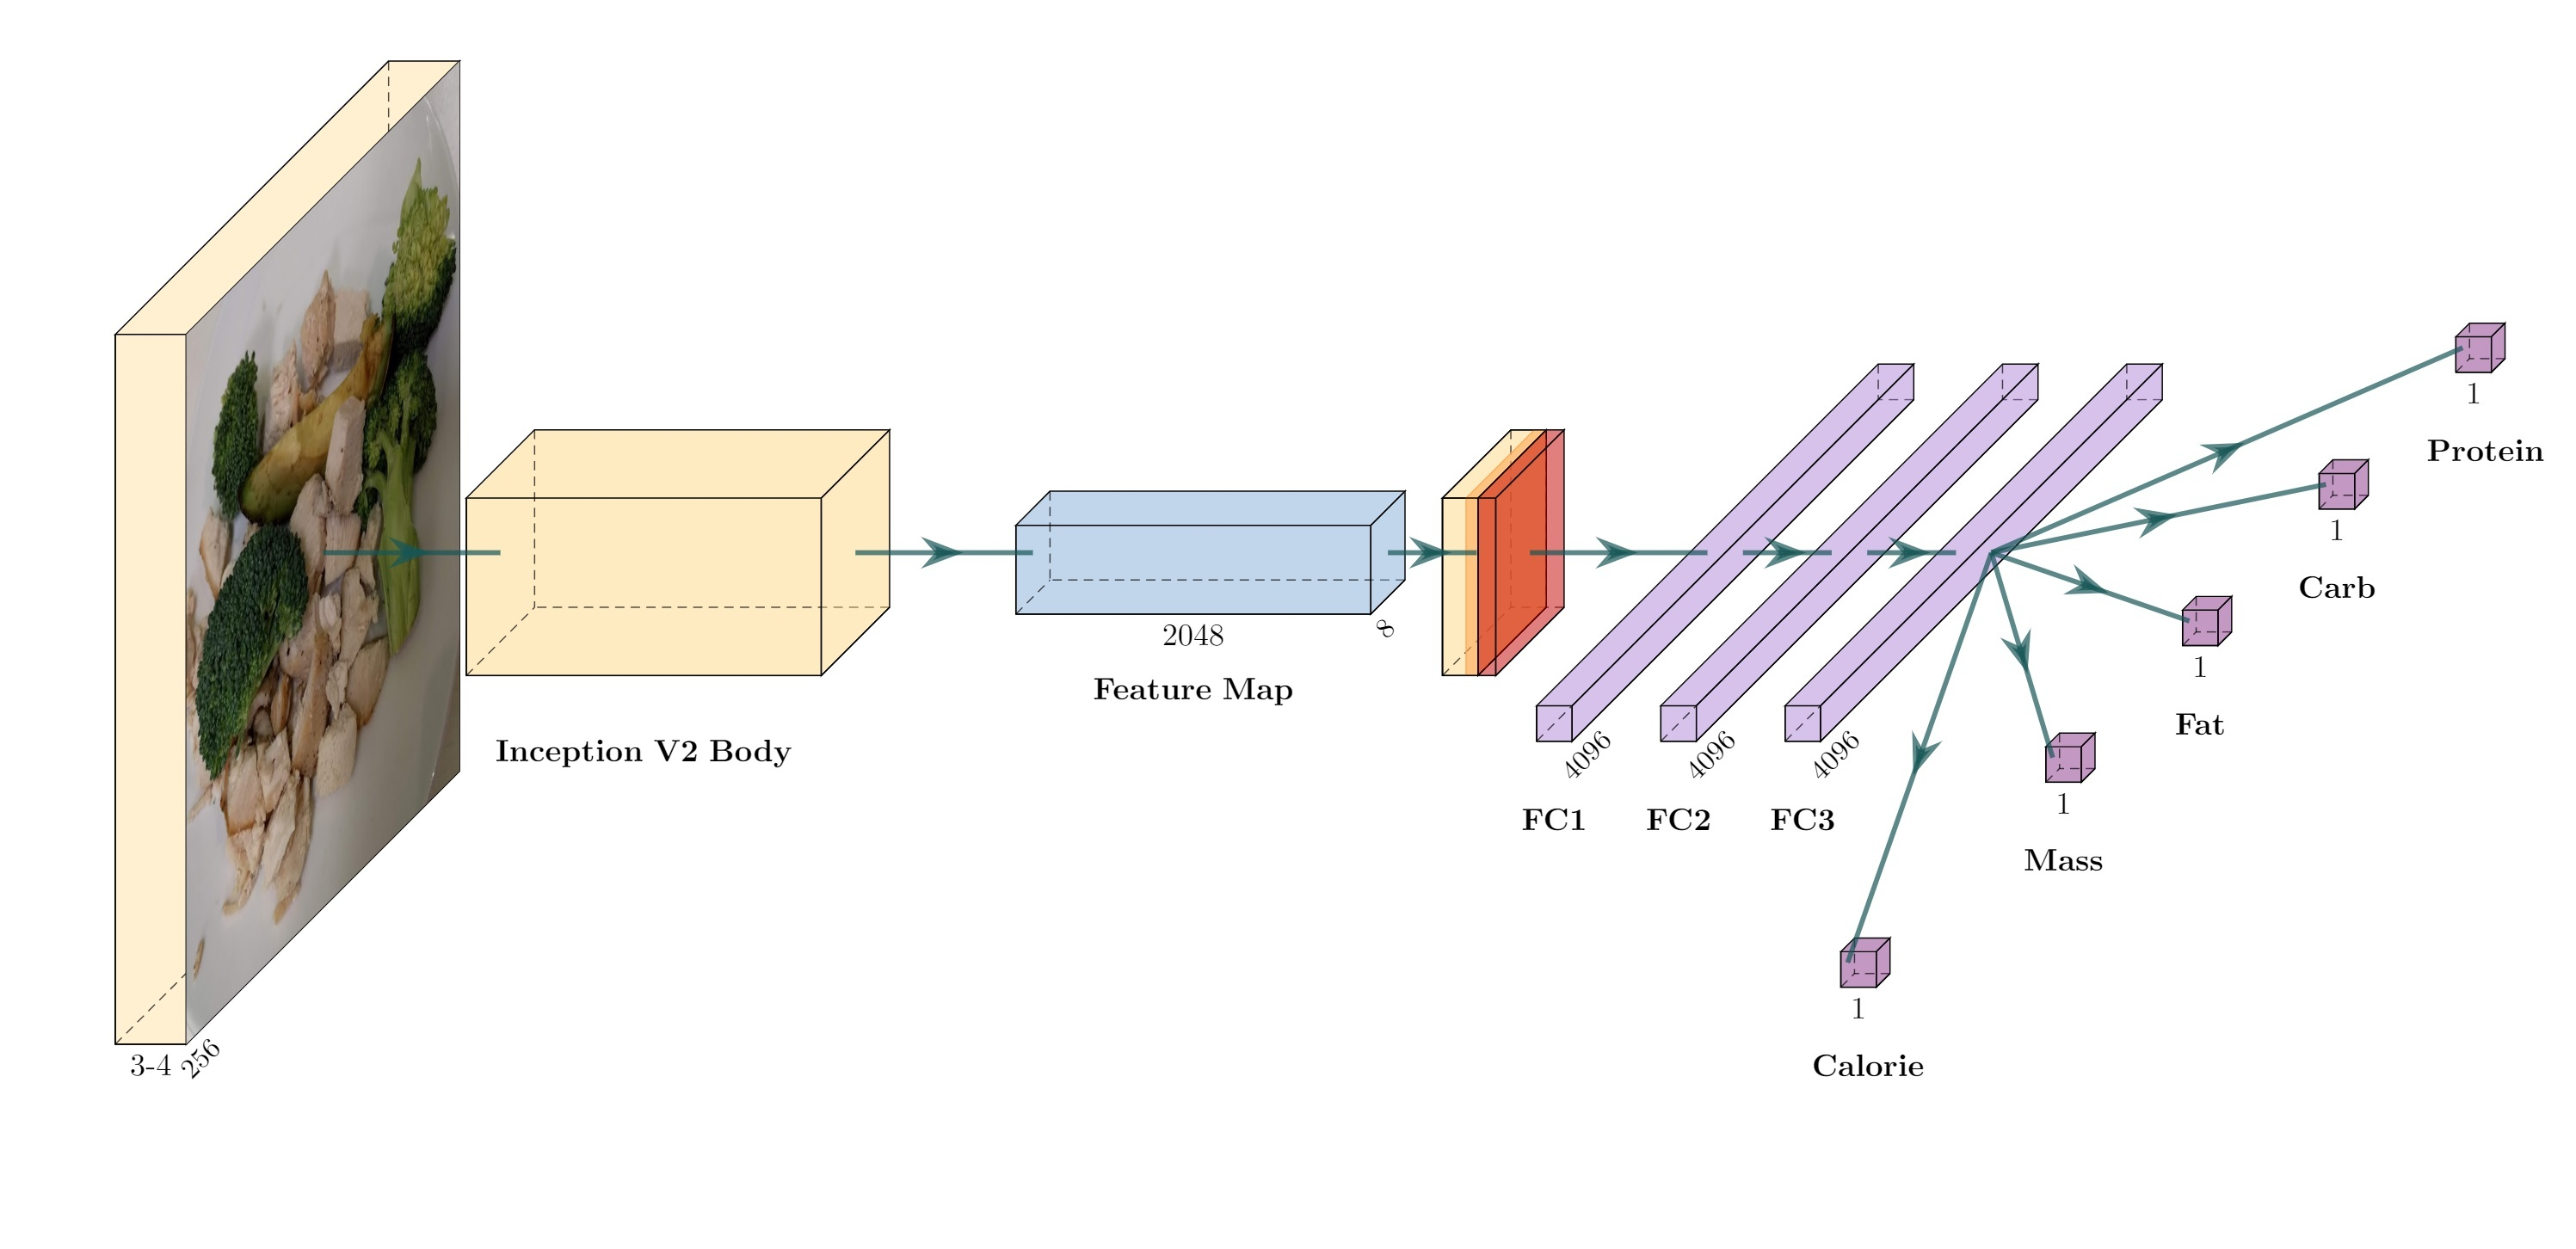
\includegraphics[width=\linewidth]{figures/literature/nutrition5k-fig6.jpg}
 \caption{Nutrition5k 的多任务回归网络。引自 Thames 等\cite{thames2021nutrition}\href{https://arxiv.org/pdf/2103.03375v2}{原图 6}（\href{https://creativecommons.org/licenses/by/4.0/}{CC BY 4.0}）。InceptionV2 后的两层 FC 共享参数，随后以独立分支预测蛋白质、碳水、脂肪、总重量和热量。}
 \label{fig:nutrition-architecture}
\end{figure}

深度信息进一步改善了份量估计。一种设置将深度作为额外通道与 RGB 联合输入；另一种设置根据相机几何和食物前景估计体积，将体积标量与 RGB 特征结合，用独立的 \textbf{InceptionV3 重量网络}预测总重量，再与每克营养密度组合。在论文表 4 的俯视重量回归实验中，图像输入基线 MAE 为 38.1 g，加入体积后降至 29.4 g，显示了几何信息对份量预测的价值。该比较对应相同的重量任务，RGB-D 研究则使用具备深度的子集。

食材组成、份量和营养密度共同决定整餐营养。单张 RGB 图像的主要困难在于尺度缺失、遮挡，以及油脂和调味料等不可见成分；Nutrition5k 集中的采集地点与视角也使跨场景推广成为重要问题。FoodLens 采用课程 RGB 数据，以\textbf{食材 F1、重量与营养 MSE、JSON/Schema 有效率}分别衡量语义、定量和结构质量。这一分层评价将两条研究路线的目标落实到同一膳食记录中，并保留各自明确的检验依据。

\FloatBarrier
\subsection{多模态预训练与参数高效微调}
\label{subsec:vlm-peft}
\flfocus{预训练模型提供图文理解基础，低秩适配与量化分别压缩任务更新规模和基础权重存储。}

\subsubsection{视觉语言基础模型的领域适配}
\textbf{Qwen3-VL}\cite{bai2025qwen} 采用视觉编码器、视觉语言映射模块与 Qwen3 语言模型组成的架构，提供 2B、4B、8B、32B 等稠密模型。其 \textbf{DeepStack} 将多个视觉编码层的特征经专门映射注入语言模型前几层，加强不同层次视觉信息的利用；交错 MRoPE 改进时空位置表示，视频时间戳提供显式时序信息。分阶段预训练与后训练进一步形成多种视觉指令的处理能力。

报告通过视觉问答、文字识别、空间理解和多模态推理基准展示通用能力，并以消融实验支持多层融合的作用。FoodLens 选择 Qwen3-VL 的依据是\textbf{图文理解与指令适配能力}：通过领域样本学习膳食字段和 JSON 输出形式，衔接通用预训练与课程任务。食物重量与营养回归属于领域目标，实际效果由课程数据上的微调前后对照检验。

图\ref{fig:qwen-architecture}呈现基础模型的实际架构：视觉编码器形成视觉 Token，语言模型处理图文序列，右侧 DeepStack 将多个视觉层的特征注入语言模型的早期层。

\begin{figure}[!htbp]
 \centering
 % Original Qwen3-VL Fig. 1 plus an explicitly marked enlargement.
% Main network is unchanged. The video-example region is replaced by the inset.
\begin{tikzpicture}
 \node[inner sep=0,anchor=south west] (original) at (0,0)
  {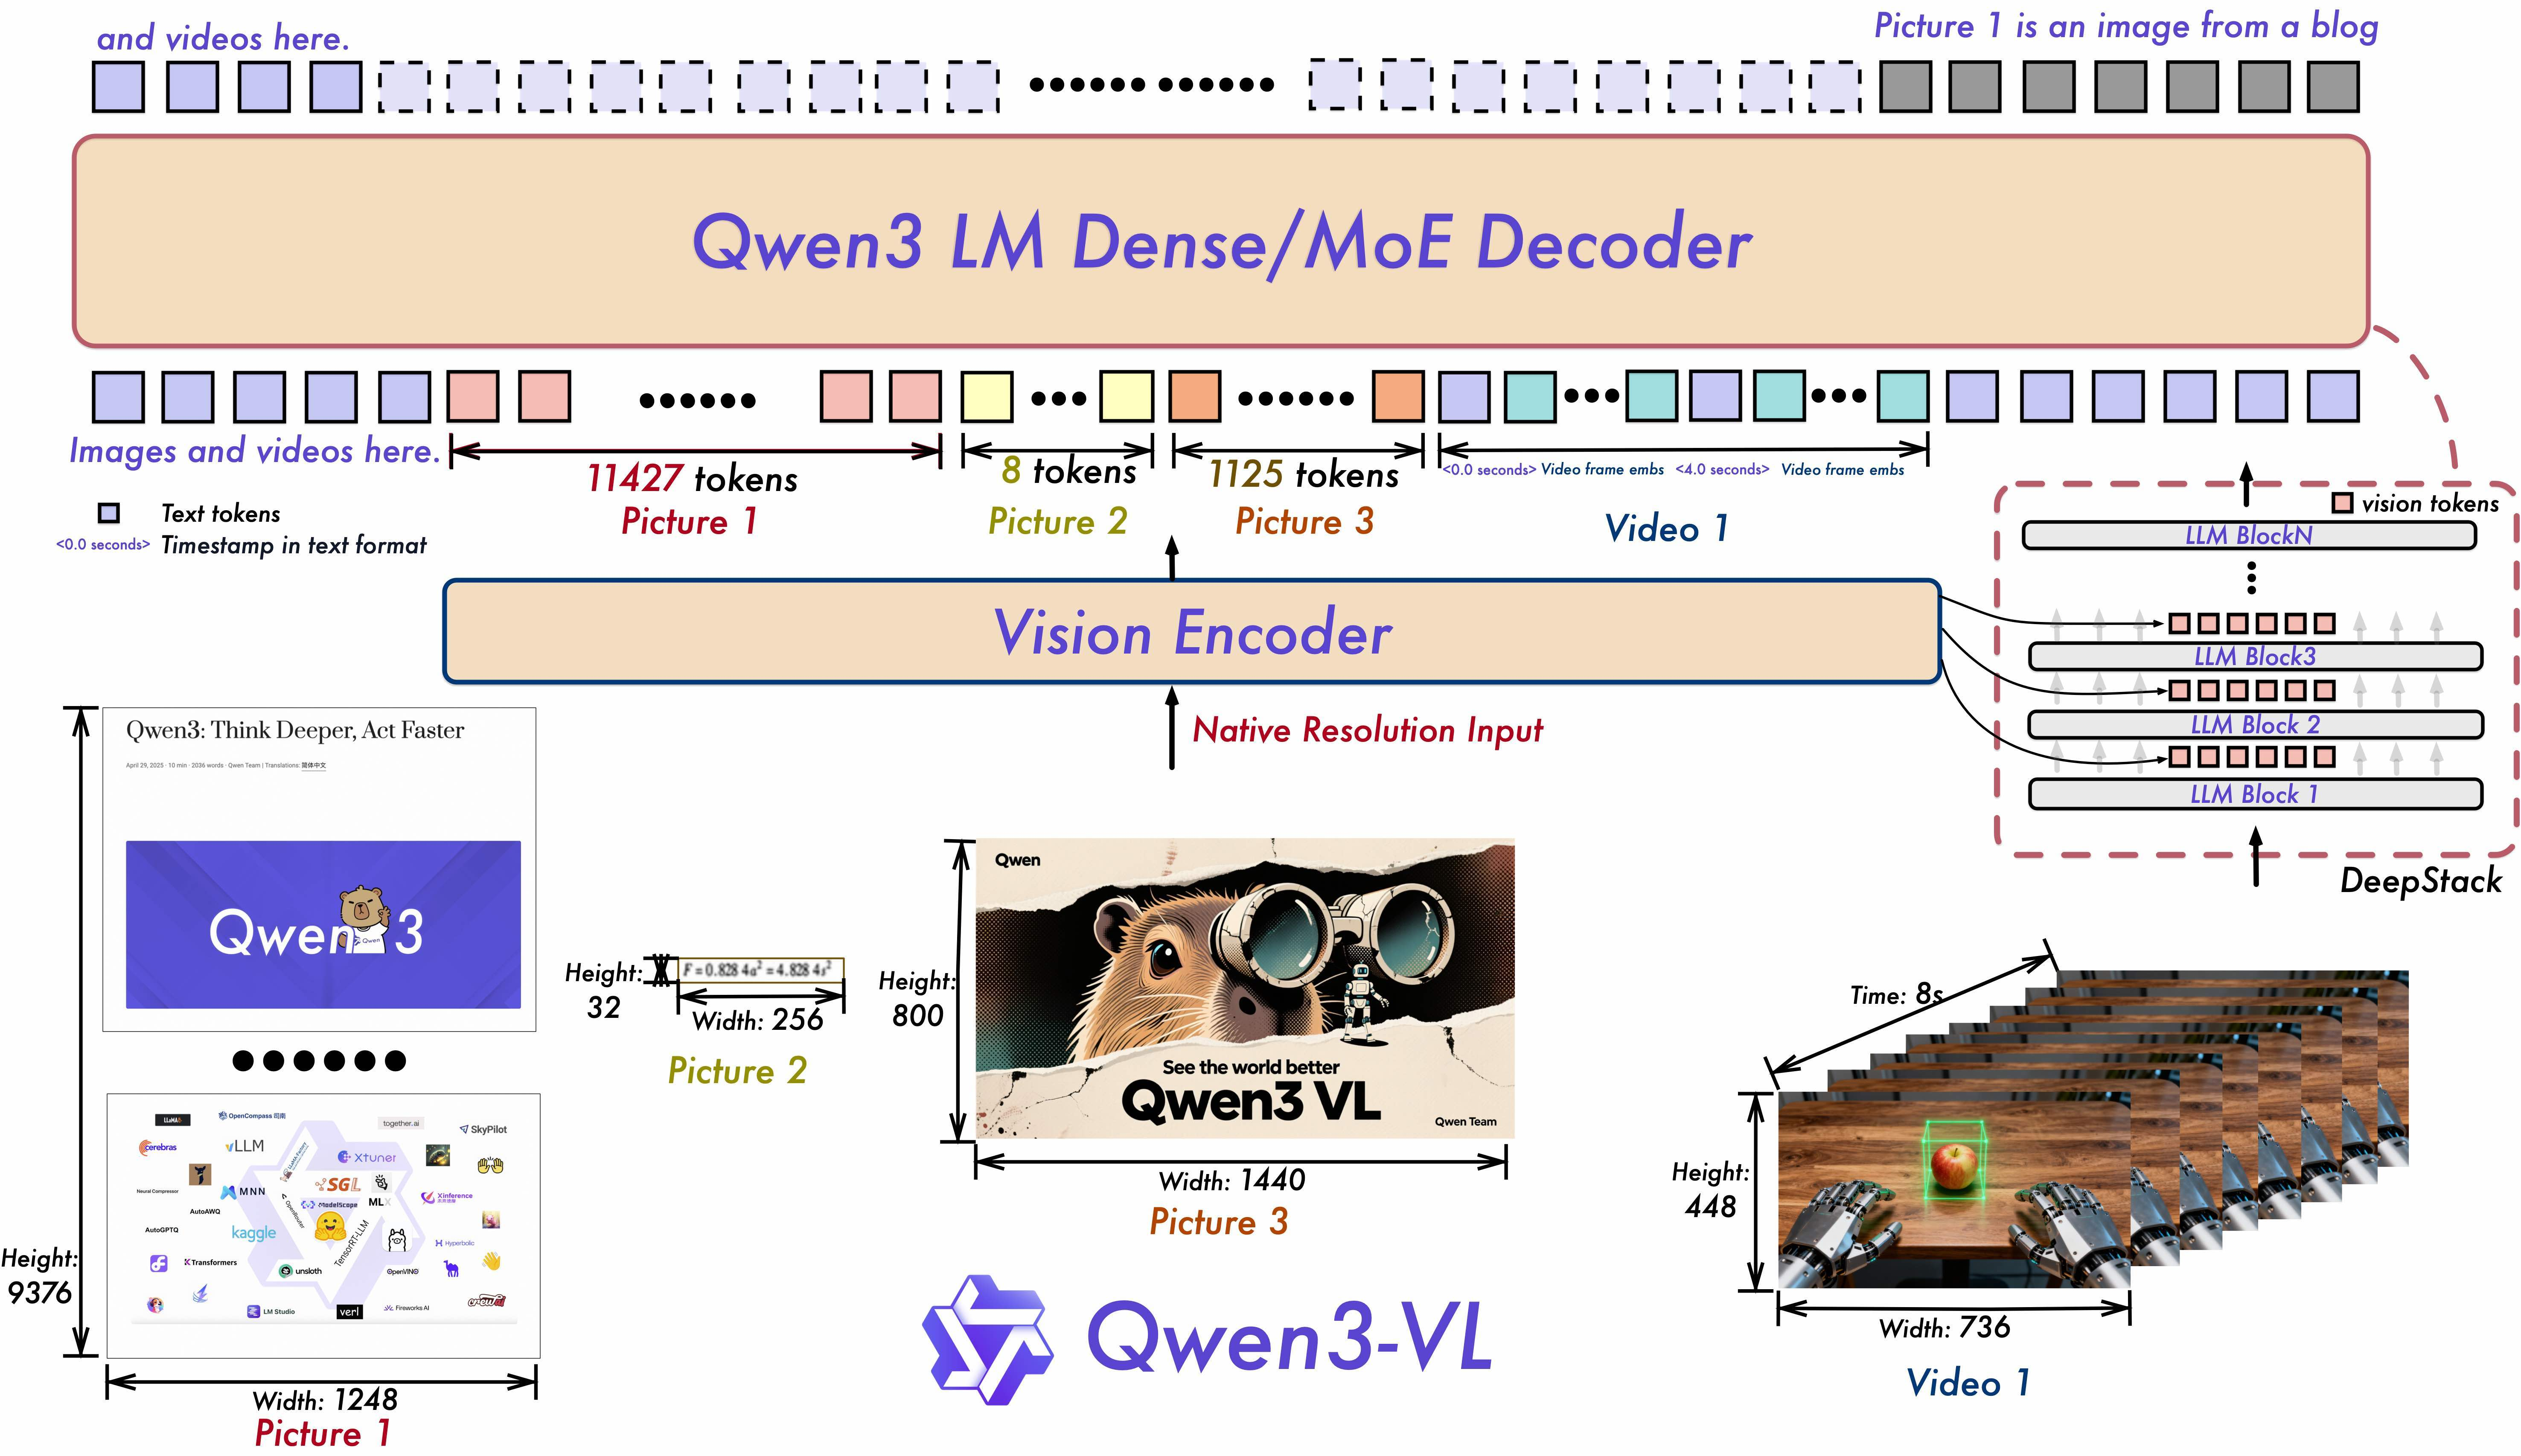
\includegraphics[width=\linewidth]{figures/literature/qwen3vl-fig1.jpg}};
 \begin{scope}[x={(original.south east)},y={(original.north west)}]
  \fill[white] (0.64,0) rectangle (1,0.415);
  \node[anchor=south east,inner sep=0] at (0.998,0.005)
   {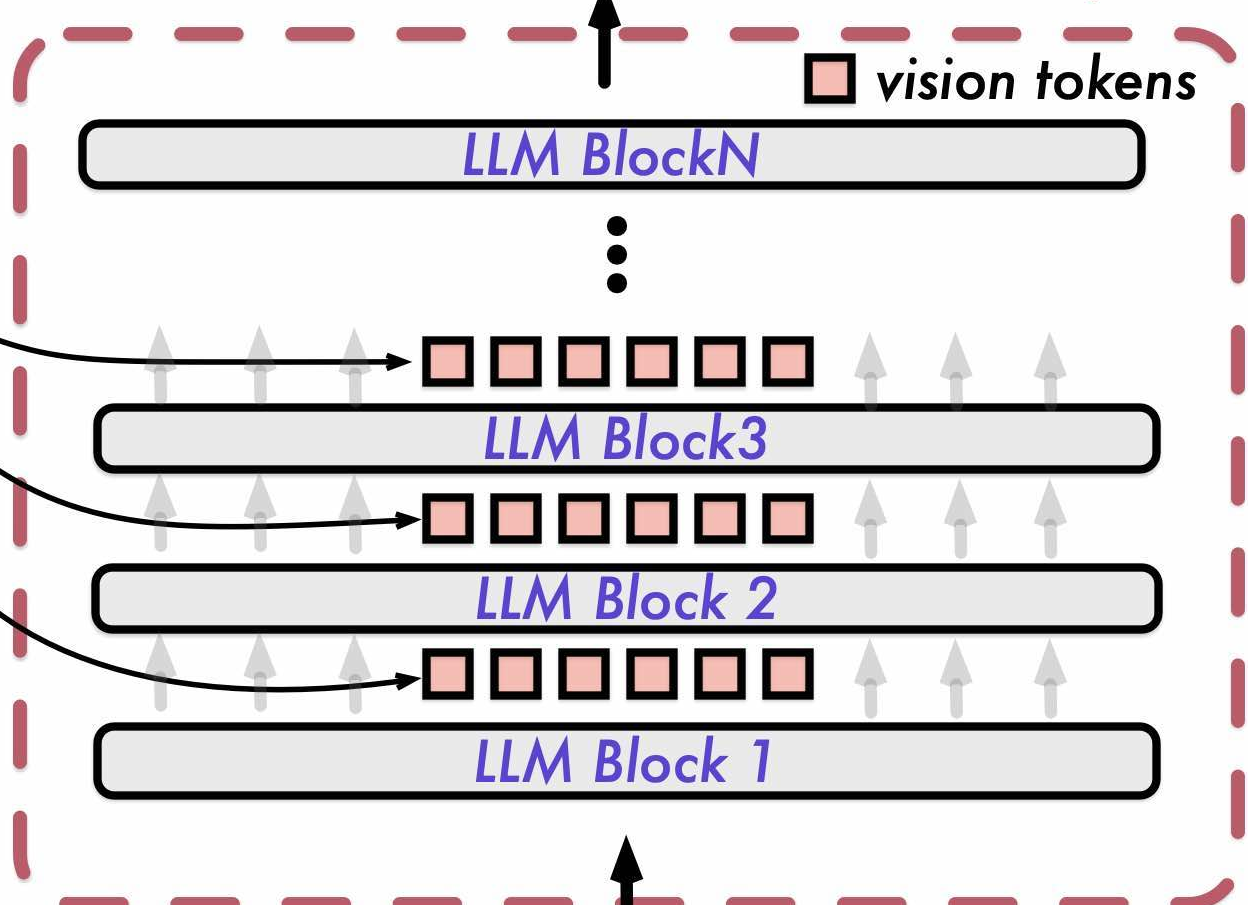
\includegraphics[width=0.30\linewidth]{figures/literature/qwen3vl-deepstack-detail.png}};
  \node[anchor=north,inner sep=0,font=\fontsize{8}{10}\selectfont\bfseries,text=FLBlue]
   at (0.825,0.409) {DeepStack 局部放大};
 \end{scope}
\end{tikzpicture}

 \caption{Qwen3-VL 的多模态基础架构。引自 Bai 等（Qwen Team）\cite{bai2025qwen}\href{https://arxiv.org/pdf/2511.21631v2}{技术报告 v2 原图 1}；右下视频输入示例替换为 DeepStack 局部放大，主体网络与连接保持原样。}
 \label{fig:qwen-architecture}
\end{figure}

\subsubsection{低秩更新与量化存储}
\textbf{LoRA}\cite{hu2022lora} 将任务适配表示为冻结基础权重上的低秩增量。对 $W_0\in\mathbb{R}^{d\times k}$，其更新形式为
\begin{equation}
 W=W_0+\frac{\alpha}{r}BA,\qquad
 B\in\mathbb{R}^{d\times r},\quad A\in\mathbb{R}^{r\times k},
 \quad r\ll\min(d,k).
\end{equation}
可训练参数由 $dk$ 降为 $r(d+k)$，其中 $r$ 控制适配容量，$\alpha$ 调节更新尺度。原论文在多种语言模型任务上获得与全量微调相当或更好的效果，并减少参数、优化器状态及训练显存开销。低秩更新可合入基础权重，便于保存与切换任务适配结果；秩与注入模块共同决定更新范围。

\textbf{QLoRA}\cite{dettmers2023qlora} 在低秩适配基础上，以 4 位形式存储冻结权重，通过反量化参与较高精度计算，将梯度传递给适配器。\textbf{NF4、双重量化与分页优化器}分别优化权重表示、量化常数存储和显存峰值。论文在特定语言模型配置下实现了单张 48 GB GPU 适配 65B 模型，并在多项实验中接近 16 位适配效果；其 33B、65B 与全量 16 位微调的效果比较仍受资源限制。

图\ref{fig:qlora-memory}从基础模型、适配器和优化器状态三个层面比较微调成本。\textbf{LoRA 减少训练更新，QLoRA 进一步压缩基础权重}，共同服务于有限算力下的领域适配。多模态训练的实际成本还取决于视觉 Token 数量、序列长度、模块选择与量化算子兼容性。FoodLens 因而同时记录显存、耗时和任务质量，以食材 F1、数值 MSE 与 Schema 有效率评价微调收益，形成资源效率与领域效果之间的对照。

\begin{figure}[!htbp]
 \centering
 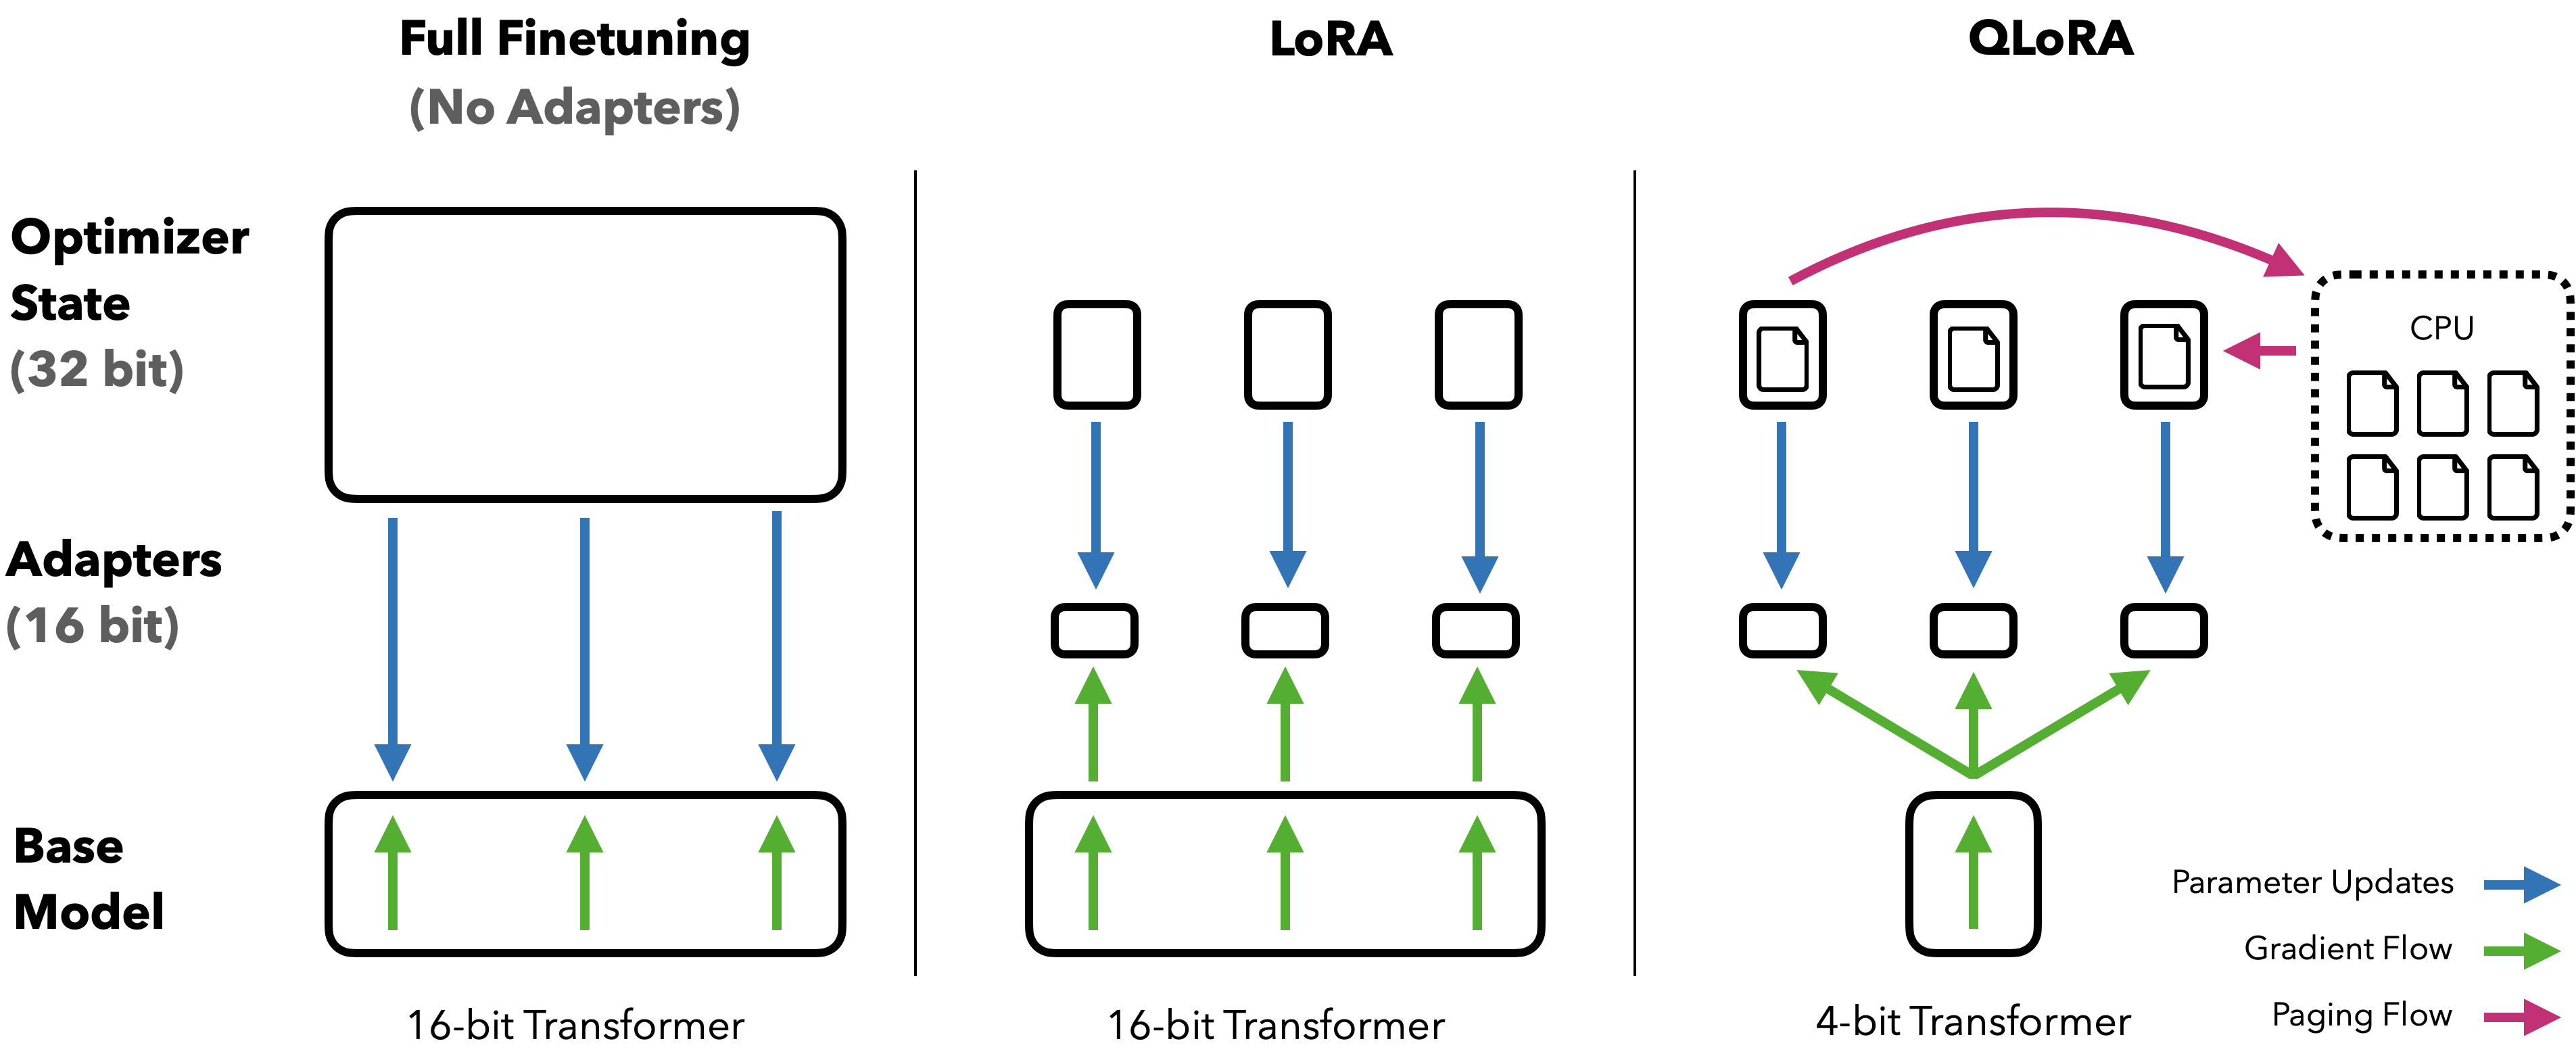
\includegraphics[width=\linewidth]{figures/literature/qlora-fig1.png}
 \caption{全量微调、LoRA 与 QLoRA 的参数更新和存储机制。引自 Dettmers 等\cite{dettmers2023qlora}\href{https://arxiv.org/pdf/2305.14314v1}{原图 1}（\href{https://creativecommons.org/licenses/by/4.0/}{CC BY 4.0}）。QLoRA 冻结 4 位基础权重，以分页优化器缓解显存峰值。}
 \label{fig:qlora-memory}
\end{figure}

\FloatBarrier
\subsection{生成模型的训练优化与评价}
\label{subsec:optimization-evaluation}
\flfocus{训练优化改变模型参数，质量评价检验输出；序列奖励将两者连接起来。}

\subsubsection{从逐词似然到序列级优化}
交叉熵训练逐词拟合参考描述，最终指标则对整句评分；Teacher Forcing 与推理使用自身前缀之间也存在条件差异。\textbf{SCST}\cite{rennie2017scst} 采用策略梯度，将采样描述的奖励与模型自身推理解码结果的奖励之差作为优势信号。经典实现以贪心解码为基线，强化优于当前推理结果的序列，直接优化 CIDEr 等不可微指标并降低估计方差。论文在 MS COCO 上验证了这一序列级优化策略。

\textbf{CIDEr 等指标既可报告质量，也可作为 SCST 奖励}，前者用于比较输出，后者参与参数更新。FoodLens 的任选实验比较交叉熵与 SCST，同时观察描述指标、食材细节和幻觉变化，以分析序列奖励带来的实际收益。

\subsubsection{从图文一致性到结构化解释}
\textbf{CLIPScore}\cite{hessel2021clipscore} 用预训练 CLIP 编码图像与候选描述，对归一化表征的余弦相似度进行截断和缩放，形成无需参考文本的图文相容性分数。论文在 Flickr8k、COMPOSITE 等人工判断数据上验证了相关性，并提出结合参考文本的 RefCLIPScore。整体语义匹配为 BLEU、CIDEr 等文本指标补充了直接的视觉依据。

\textbf{FLEUR}\cite{lee2024fleur} 将图像、候选描述和评分标准输入 LLaVA，通过追加提示解释分数。其分数平滑使用小数位数字 Token 的概率计算加权期望，缓解离散打分中的大量并列。该方法在 Flickr8k-CF、COMPOSITE、Pascal-50S 等设置中表现出较好的人工判断一致性，将无参考评价扩展为\textbf{可阅读的评分依据}；概率平滑依赖可访问的模型输出概率。

\textbf{EXPERT}\cite{kim2025expert} 进一步以流畅性、相关性、描述充分性组织解释，在人工评分数据基础上构建解释监督，并以先评分、后解释的模板微调视觉语言模型。它分别检验评分相关性和解释的一致性、事实性、信息量，实验支持\textbf{统一标准与解释监督的结合}能够改善解释质量。其在多数无参考基准上取得较好结果，Pascal-50S 部分设置由其他方法领先；原文误差分析还指出了对细节缺失惩罚过重的情形。

表\ref{tab:evaluation}归纳了各方法的角色。多模态评价的共同挑战是视觉判断偏差、解释可靠性和推理成本。FoodLens 的 VLM-as-Judge 参考 FLEUR 的视觉条件评分与 EXPERT 的结构化解释，通过人工样本检查食材误判、遗漏和幻觉，形成与传统自动指标互补的分析。\textbf{食材识别与营养数值}分别由任务指标检验，使语言质量、视觉事实和定量误差各有依据。

\begin{table}[!htbp]
 \caption{训练优化与无参考评价方法的角色比较}
 \label{tab:evaluation}
 \centering\small
 \setlength{\tabcolsep}{5pt}\renewcommand{\arraystretch}{1.16}
 \begin{tabularx}{\linewidth}{@{}P{2.1cm}P{2.65cm}YP{3.4cm}@{}}
 \toprule
 \textbf{方法} & \textbf{方法类别} & \textbf{主要用途} & \textbf{FoodLens 对应任务}\\
 \midrule
 SCST & 序列级训练优化 & 用奖励差更新生成策略 & 任选：描述模型继续训练\\
 CLIPScore & 图文相似度评价 & 衡量整体语义相容性 & 描述质量的补充指标\\
 FLEUR & 多模态无参考评价 & 概率平滑评分、自然语言解释 & 任选：视觉评分与错误解释\\
 EXPERT & 监督适配的无参考评价 & 标准化、多维度解释 & 任选：结构化评价与人评校准\\
 \bottomrule
 \end{tabularx}
\end{table}

\FloatBarrier
\subsection{本章小结}
图像描述研究沿着\textbf{全局表示—空间选择—视觉关系与跨层融合}发展，Food-500 Cap 将这些方法的检验落到菜品和可见属性。结构化膳食研究进一步揭示了食材语义、份量监督与营养密度之间的联系。单图尺度和不可见成分是定量预测的核心困难，领域差异与评价偏差则贯穿模型迁移和结果分析。

FoodLens 的技术选择由此形成清晰对应：以 \textbf{ResNet-18 + GRU、ResNet Grid + Transformer}比较视觉表示与生成方式，以 Qwen3-VL + LoRA/QLoRA 研究结构化膳食适配，以 SCST 检验序列优化收益，以 VLM-as-Judge 增强评价解释。项目围绕自主实现、预训练适配与对照分析展开，分别检验描述、食材、数值与结构质量，体现对相关方法的理解及其在课程条件下的工程实现能力。
